%% This is an example first chapter.  You should put chapter/appendix that you
%% write into a separate file, and add a line \include{yourfilename} to
%% main.tex, where `yourfilename.tex' is the name of the chapter/appendix file.
%% You can process specific files by typing their names in at the 
%% \files=
%% prompt when you run the file main.tex through LaTeX.
\chapter{Results and Testing}
This chapter will describe the results of my work with of W. A. Mozart's \textit{Eine kleine Nachtmusik, K.525} as an exmaple. This chapter will also look at timing metrics of the system.

\section{An Example: Eine kleine Nachtmusik, K.525, W. A. Mozart)}
This section will go through an example of how the entire \texttt{OMRMIDICorrector} system works on W. A. Mozart's \textit{Eine kleine Nachtmusik, K.525}.

\begin{figure}[H]
\centering
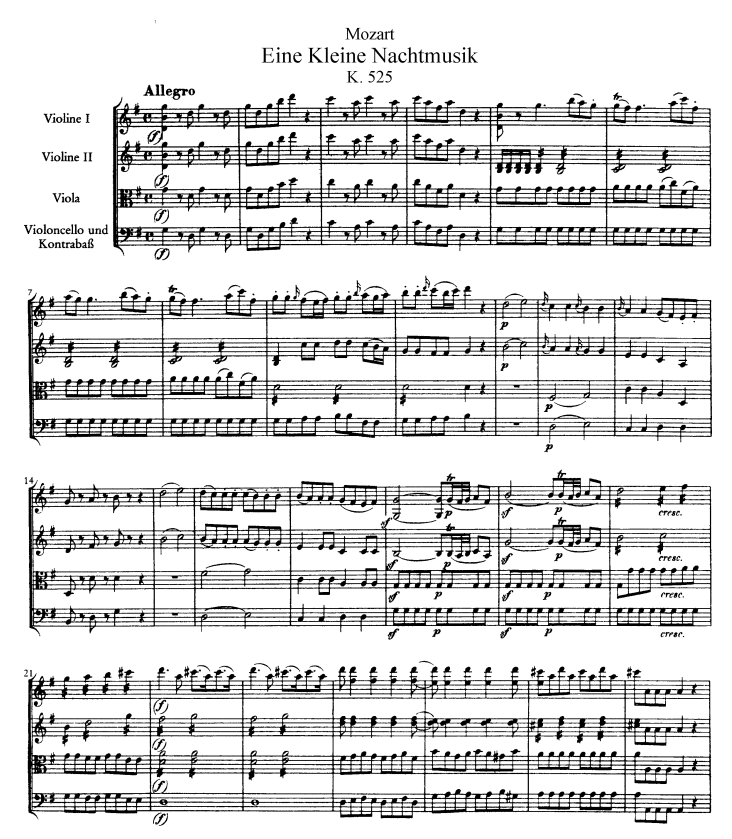
\includegraphics[width =.9\textwidth]{k525originalomrscan}
\caption{The first page of the scanned copy of the score found on IMSLP.}
\end{figure}

\subsection{Musical Properties of K.525}
I chose K.525 as the example piece for many of it music properties that make it a difficult but interesting piece to align and correct. In the hashing, align

\subsubsection{Bass and Cello Doubling}
In the original scanned score, there are only four parts because the bass part doubles the cello part one octave lower. However, in the MIDI encoding, there must be five separate voices. Thus, in the preprocessing step of the \texttt{OMRMiDICorrector}, it would be ideal for the system to recognize this. Otherwise, in instances where the \texttt{OMRMIDICorrector} could not pair up the parts between the input OMR stream and the input MIDI stream, there would be an error thrown, and alignment and correction would not happen. 

\subsubsection{Tremolos}
Starting in measure 5 in the original scanned score, the second violin has tremolo notes, instead of repeated \nth{16} notes written out. The OMR parser in SmartScore is not robust enough to recognize the slashes across the stem of the note as tremolo markings and instead interprets it as a single note. The MIDI protocol has no way of indicating tremolos, so the second violin's notes in measure 5 are encoded as regular \nth{16} notes. Ideally, the aligner would be robust enough to align tremolo measures with non-tremolo measures even though there will be a huge discrepancy in the number of notes present in the measure.

\subsection{Preparing the Raw Input}
The basic raw input of the system is an OMR score and a MIDI file. A scanned copy of the score was found in IMSLP \cite{k525}, the source for much free public domain sheet music. The MIDI file was sourced from the Yale MIDI Archive. 

\begin{figure}[H]
\centering
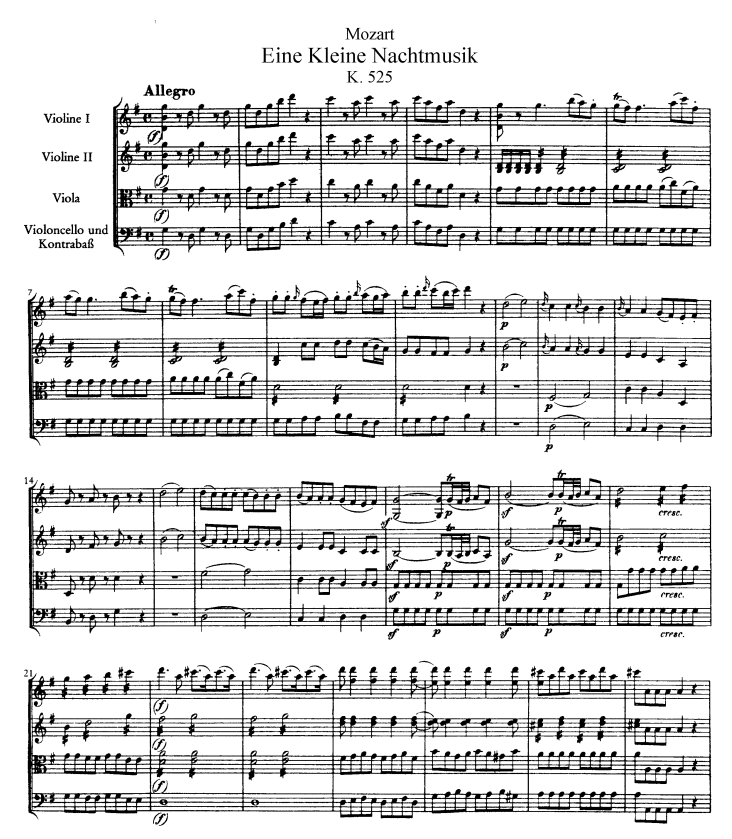
\includegraphics[width =.9\textwidth]{k525originalomrscan}
\caption{The first page of the scanned copy of the score found on IMSLP.}
\end{figure}

I used SmartScore's built-in OMR tool to convert the scanned score of K.525 into an ENF file. Then I exported the post-OMR file as a musicXML file.

Similarly for the K.525 MIDI file, I used SmartScore to parse the original file and exported it as a musicXML file. 

The last step of preparing the raw input is to parsing the musicXML files with the \texttt{music21} library so that they are \texttt{Stream} objects. This can be done by passing in the musicXML filepaths to the \texttt{parse} method in the \texttt{converter} class. We will call these two parsed streams \texttt{k525midiStream} and \texttt{k525omrStream}. 

\subsection{Running OMRMIDICorrector on K.525}

\section{Timing} \label{timing}

